%%
%% Template thesis.tex
%%
\documentclass[twoside,doublespace,onecolumn,11pt,a4paper]{book}
\usepackage[palatino]{StyFiles/anuthesis}
\usepackage{graphicx}
\usepackage{StyFiles/thesis}
\usepackage{makeidx}
% \usepackage{StyFiles/doublespace}

% Chuck Added
\usepackage[toc,page]{appendix}
\usepackage{StyFiles/fancyhdr}
% Gould Configurations

% For figures
% \ifCLASSINFOpdf
% \usepackage[pdftex]{graphicx}
% \DeclareGraphicsExtensions{.jpg,.png}
% \else
% \usepackage[dvips]{graphicx}
% \DeclareGraphicsExtensions{.eps}
% \fi

% For citations
\usepackage[sort,numbers]{StyFiles/natbib}
\renewcommand{\citename}{\citet}
\renewcommand{\cite}{\citep}
\usepackage{StyFiles/natbibspacing}

% For maths
\usepackage[cmex10]{amsmath}
\usepackage{amssymb,amsthm}

% For algorithms
\usepackage{StyFiles/algorithm}
\usepackage{StyFiles/algorithmic}

% For Hyperlinks
\usepackage{hyperref}
% fix problem between hyperref and algorithmic
\newcommand{\theHalgorithm}{\arabic{algorithm}}

% For captions
\usepackage[font=small,labelfont=bf]{caption}
\usepackage[font=footnotesize]{subfig}

% My macros
\usepackage{StyFiles/sg-macros}

\newtheorem{thm}{Theorem}[section]
\newtheorem{cor}[thm]{Corollary}
\newtheorem{lem}[thm]{Lemma}
\newtheorem{prop}[thm]{Proposition}
\newtheorem{obs}[thm]{Observation}
\newtheorem{defn}[thm]{Definition}

\newcommand{\mmqp}[3]{\textrm{\sc MaxMarginQP}\!\left(\{\by_t, #1\}_{t=1}^{T}, #2, #3\right)}

% correct bad hyphenation here
\usepackage{StyFiles/hyphenat}
\hyphenation{op-tical net-works semi-conduc-tor}


%%%%%%%%%%%%%%%%%%%%%%%%%%%%%%%%%%%%%%%%%%%%%%%%%%%%%%%%%%%%%%%%%%%%%%%
%% Preamble
\title{Latent Structural SVM Learning for Lower Linear
  Envelope Potentials in Binary Markov Random Fields}
\author{Chang Li} \date{\today}

\renewcommand{\thepage}{\roman{page}}

\makeindex
\begin{document}



\section{MISC}
\label{sec:MISC}

\subsection{Alternative QP Formulations}

We can take this process one step further and represent the
higher-order potential as with non-negativity constraints on
$\theta''_k$ for $k = 2, \ldots, K$, and appropriate feature
vectors, \ie

Here we are encoding the coefficients of the pseudo-Boolean
function used during inference directly into the learning
problem. Like the previous formulation we know that the optimal
$b_1$ is zero so can simply drop $\theta_0$ and $\phi_0$ from the
optimization.

It is interesting to note the resemblance of the latter QP
formulation with latent-variable structural SVM
learning~\cite{Yu:ICML09}.

In our formulation the auxiliary variables $\bz$ (see
\secref{sec:exact_inference}) can be determined directly from the
ground-truth or inferred labels $\by$. Moreover, since we have
fixed the piecewise-linear approximation to have equally spaced
break-points, the auxiliary variables are independent of the
parameters $(a_k, b_k)$ given $\by$. We also have that the $b_k$
are a function of the $a_k$ (by \eqnref{eqn:bk}). Removing the
restriction of equally spaced break-points (and introducing the
$b_k$ into the optimization) results in a latent-variable SVM.
The main difficulty is that the latent variables $\bz$ now depend
on the parameters making the optimization problem non-convex.

A number of other variants can be considered by linearly
constraining $\btheta$ (or alternatively re-defining
$\phi(\by)$). For example, the parameters of the $P^{n}$-model
can be learned by constraining $\theta_0 \leq \theta_1$ and
forcing $\theta_i = \theta_{i-1}$ for $i = 2, \ldots, K - 1$.
Although this case is somewhat uninteresting as there is only one
parameter to learn (since by Observation~\ref{obs:b0} we can set
$\theta_1 = \ldots = \theta_K = 0$ without changing the shape of
the potential function), which can often be done more efficiently
by other means, \eg cross-validation over a range of values.



\subsection{Algorithm}
\label{sec:MISC}

\begin{theorem}
  For the setting $\epsilon = 0$, \algref{alg:learning} terminates
  with the optimal parameters $\btheta^\star$ for
  $\mmqp{\Y_t}{\bD^2}{\zeros}$.
  \label{thm:learning}
\end{theorem}
%
\begin{proof}
  By Theorem~\ref{thm:inference}, our test for the most violated
  constraints (lines 7 and 8) can be performed exactly ($\Delta(\by,
  \by_t)$ decomposes as a sum of unary terms). If the test succeeds,
  then $\by_t^\star$ cannot already be in $\A_t$. It is now added
  (line 9). Since there are only finitely many constraints, this
  happens at most $2^n - 1$ times (per training example), and the
  algorithm must eventually terminate. On termination there are no
  more violated constraints, hence the parameters are optimal.
\end{proof}
\bigskip

Unfortunately, as our proof suggests, it may take exponential time for
the algorithm to reach convergence with $\epsilon =
0$. \citename{Tsochantaridis:JMLR05} showed, however, that for
$\epsilon > 0$ and no additional linear constraints (\ie $\bG =
\zeros$, $\bh = \zeros$) max-margin learning within a dual
optimization framework will terminate in a polynomial number of
iterations. Their result can be extended to the case of additional
linear constraints (see the Appendix for details).

\subsection{Max-margin Learning}
%
Given an energy function $\energy{\by; \btheta} = \btheta^T \!
\phi(\by)$ parameterized as a linear combination of features
$\phi(\by) \in \reals^m$ and weights $\btheta \in \reals^m$, and
a set of $T$ training examples $\{\by_t\}_{t=1}^T$ the max-margin
framework is a principled approach to learning the weights of the
model.

In our formulation we will allow additional linear constraints to
be imposed on the weights of the form $\bG \btheta \geq \bh$,
where $\bG \in \reals^{d \times m}$ and $\bh \in \reals^d$. This
is not typically necessary for max-margin learning, but, as we
will see below, is required for enforcing concavity when learning
lower linear envelope potentials.

Now, let $\Y_t = \{0, 1\}^n$ be the set of all possible
assignments for the $t$-th training example. The
(margin-rescaling) max-margin approach formulates learning as a
quadratic programming optimization problem,
$\mmqp{\Y_t}{\bG}{\bh}$:
%
\begin{align}
  & \textrm{minimize} \quad \textstyle \frac{1}{2} \|\btheta\|^2 + \frac{C}{T} \sum_{t=1}^{T} \xi_t
  \label{eqn:maxmarginqp} \\
  & \textrm{subject to} \notag \\
  & \begin{array}{lll}
    & \btheta^T \delta\phi_t(\by) + \xi_t \geq \Delta(\by, \by_t), & \forall t, \by \!\in\! \Y_t, \\
    & \xi_t \geq 0, & \forall t, \\
    & \bG \btheta \geq \bh
  \end{array} \notag
\end{align}
%
where $\delta\phi_t(\by) \triangleq \left(\phi_t(\by) -
  \phi_t(\by_t)\right)$ is the difference between feature
representations for some assignment $\by$ and the $t$-th
ground-truth assignment $\by_t$, $C > 0$ is a regularization
constant, and $\Delta(\by, \by_t)$ measures the loss between a
ground-truth assignment $\by_t$ and any other assignment. In our
work we use the Hamming loss, which measures the proportion of
variables whose corresponding assignments disagree. More
formally, the Hamming loss is defined as $\Delta(\by, \by') =
\frac{1}{n} \sum_{i=1}^{n} \ind{y_i \neq y'_i}$, where $\ind{P}$
is the indicator function taking value one when $P$ is true and
zero otherwise.

The number of constraints in the QP is exponential in the number
of variables, and a standard approach to solving the max-margin
QP is by adding constraints incrementally. Briefly, at each
iteration the algorithm checks for the most violated constraint
(for each training example), using \emph{loss-augmented
  inference}, and, if found, adds it to the constraint set. The
algorithm terminates when no more violated constraints are found
(see \algref{alg:learning}).



\subsection{Weighted Lower Linear Envelope Potentials}

Suppose we have a binary MRFs $\mathbf{y}=\{y_1,\dots,y_n\}$,
$y_i\in\{0,1\}$. A higher-order potential
$\psi_c^H(\mathbf{y}_c)$ is an arbitrary function defined on
cliques $\mathbf{y}_c=\{y_i : i\in c\}$ where
$c\subseteq\{1,\dots,n\}$. Gould\cite{gouldlearning} proposed it
with a weighted lower linear envelope potential expression

\begin{align}
  \psi_c^H(\mathbf{y}_c) \triangleq
  \min_{k=1,\dots,K}\bigg\{a_kW_c(\mathbf{y}_c)+b_k\bigg\}
\end{align}

where $(a_k,b_k)\in\mathbb{R}^2$ are linear function parameters
and

$$
W_c(\mathbf{y}_c) = \sum_{i\in c}^{}w_i^cy_i
$$

where c is a clique. $w_i^c$ is a per-variable non-negative
weights for every nodes in each clique and satisfies $\sum_ {i\in
  c}^{}w_i^c=1$.

In the literature they explored many important properties of
lower linear envelope. They proved that by maitaining the order
of variables $a_k$ and $b_k$, the encoding is ensured free of
redundant linear functions (Proposition 3.1\cite{gouldlearning}):

\begin{align}
  a_k > a_{k+1}\\
  b_k < b_{k+1}
\end{align}

Another important property is that the inferenced assignment
$y^*$ is irrelevant of arbitrarily shifting the piece-wise
functions set up or down. Let $ \tilde{\psi}_c^H(y_c) =
\min_{k=1,\dots,K}{a_kW_c(y_c)+b_k+b^{const}}$. We can get:

$$
arg\min_{y_c}{\psi_c^H(y_c)}=arg\min_{y_c}{\tilde{\psi}_c^H(y_c)}
$$

Therefore, we can shift arbitrary envelope to zero:

\begin{align}
  b_1 = 0
\end{align}

From equation (3) we know that variable $b_k$ maintaining
increasing order, thus $b_k>0$ when $k>1$.

To help with exact inference on the envelope,
Gould\cite{gouldlearning} rewrite it into a quadratic
pseudo-Boolean function by introducing $K-1$ auxiliary binary
variables $\mathbf{z} = {z_1,\dots,z_K-1}$:

\begin{align}
  E^c(y_c,z)=a_1W_c(y_c)+b_1+\sum_{k=1}^{K-1}z_k((a_{k+1}-a_k)W_c(y_c)+b_{k+1}-b_k)
\end{align}

It is worth to notice that as long as we maintain the linear
constraints on variables $a_k$ and $b_k$, the following
constraint is automatically satisfied (Observation
3.6\cite{gouldlearning}):

\begin{align}
  z_{k+1}\le z_k
\end{align}

In the literature they also proved the submodularity of equation
(5) and proposed a graph-cuts method to perform the exact
inference on it. Our work is based on these results.


\section{Related Work}
\subsection{MRF}
Learning structural objects from unknown probability distribution
is becoming popular in recent years.
\citename{tsochantaridis2005large} generalized multiclass
SVMs\cite{crammer2002algorithmic} to structural SVMs by extending
feature vectors to joint feature vectors which map features
extracted jointly over input-output pairs to discrete output. The
exact maximum a posteriori (MAP) problem thus becomes an NP-hard
problem. They overcome this by generalize the hard margin into
"soft" margin and found an upper bound of arbitrary loss
functions under this formulation.

Based on the previous research, \citename{yu2009learning}
developed latent SVM by introducing a hidden variable into the
joint feature vector. They observed a fact that in real world
applications hidden variables are usually intermediate results
and are not required as an output. With this fact they followed
“Soft-Margin” method and found an upper bound for the loss
function with latent variables. However, the resulted object
function is still non-convex.

\citename{yuille2002concave} developed the Concave-Convex
Procedure (CCCP) which is guaranteed to find a local minimum for
a Difference-Convex (DC) program. \citename{yu2009learning}
combined CCCP algorithm by writing their non-convex object
function into a difference of two convex functions and came up
with an EM like 2 steps optimizing algorithm. For each iteration,
they first compute latent variables utilizing current parameter
vectors and then in turn optimizing parameter vectors using the
standard Structural SVM algorithm with previously computed latent
variables.

Higher order potentials are raising interests due to their
capability to represent dependencies between complex objects.
\citename{kohli2009robust} proposed a method to represent a class
of higher order potentials with lower (upper) linear envelope
potentials. By introducing auxiliary variables, they reduced the
linear representation to a pairwise form and proposed an
approximate algorithm with standard linear programming methods.
Following their routine, \citename{gouldlearning} extended their
method to a weighted lower linear envelope in binary Markov
Random Fields (MRF) which can be solved with an efficient
algorithm. They showed the energy function with auxiliary
variables is submodular by transforming it into a quadratic
pseudo-Boolean form and how “graph-cuts” like algorithm can be
applied to do exact inference. They then optimized the model’s
parameters under the max margin
framework\cite{tsochantaridis2005large}.

In their work they pointed out the potential relationship between

their auxiliary representation and latent
SVM\cite{yu2009learning}. However, since removing of their fixed
space constraint will result dependence between latent variable
and parameters, further research still remains open.

This report will study the latent variable formulation of their
energy function and optimize it using latent SVM framework. The
rest of report is organized as follows: Section 2 gives a briefly
introduction of Latent Structural SVM. Section 3 presents the
formulation of weighted lower linear envelope potential and its
most important properties. Section 4 describes the linear
combination formulation of the energy function and how to
optimize it using latent structural SVM. Section 5 discusses its
performance on synthetic data.


\subsection{Exact Inference}
\label{sec:exact_inference}

Importantly, $E^c(\by_c, \bz)$ is a \emph{submodular} energy
function, which allows us to perform efficient inference by
minimizing jointly over both variables $\by_c$ and auxiliary
variables $\bz$.

It is well known that submodular pairwise energy functions can be
minimized exactly in time polynomial in the number of variables
by finding the minimum-$st$-cut on a suitably constructed
graph~\cite{Kolmogorov:PAMI04, Hammer:1965}. We illustrate one
possible construction for $E^c(\by_c, \bz)$ in
\figref{fig:stmincut}.


Using this fact, we can show that an energy function containing
arbitrary weighted lower linear envelope potentials can be
minimized in polynomial time.

Then $\energy{\by}$ can be minimized in time polynomial in the
number of variables $n$ and total number of linear envelope
functions. Each higher-order term adds $K - 1$ auxiliary
variables so the total number of variables in the augmented
energy function is less than $n$ plus the total number of linear
functions.

\subsection{Interactive Figure-Ground Segmentation}

We also ran experiments on the real-world ``GrabCut'' problem
introduced by~\citename{Rother:SIGGRAPH04}. Here the aim is to
segment a foreground object from an image given a user-annotated
bounding box of the object (see %\figref{fig:grabcut_results}(a)
for some examples). To solve this problem the GrabCut algorithm
associates a binary random variable $y_i$ with each pixel in the
image indicating whether the pixel belongs to the ``background''
(binary label 0) or the ``foreground'' (binary label 1).
Variables corresponding to pixels outside of the user-annotated
bounding box are automatically assigned a label of zero (\ie
background). The assignment for the remaining variables, \ie
those within the bounding box, is inferred.

We compare a model with learned higher-order terms against the
baseline GrabCut model by performing leave-one-out
cross-validation on a standard set of 50 images
from~\citename{Lempitsky:ICCV09}. Following the approach of
\citename{Rother:SIGGRAPH04}, our baseline model contains unary
and pairwise terms. The unary terms are defined as the
log-likelihood from foreground and background Gaussian mixture
models (GMMs) over pixel colour and are image-specific. Briefly,
the GMMs are initialized by learning foreground and background
models from pixels inside and outside the user-annotated bounding
box, respectively. Next, the GMMs are used to relabel pixels
(within the bounding box) as either foreground or background by
taking the label with highest likelihood according to the current
parameter settings. Next the parameters of the foreground and
background colour models are re-estimated given the new labeling.
This process of parameter estimation and re-labeling is repeated
until convergence (or a maximum number of iterations is reached).
The final GMMs are used to construct the unary terms.

The pairwise terms encode smoothness between each pixel and its
eight neighbours, and are defined as
%
\begin{align}
  \psi^P_{ij}(y_i, y_j) &= \frac{\lambda}{d_{ij}} \ind{y_i \neq y_j} \exp\left\{- \frac{\|x_i - x_j\|^2}{2 \beta}\right\}
\end{align}
%
where $d_{ij}$ is the distance between pixels $i$ and $j$, $x_i$
and $x_j$ are the RGB colour vectors for pixels $i$ and $j$,
$\beta$ is the average squared-distance between adjacent RGB
colour vectors in the image, and $\lambda$ determines the
strength of the pairwise smoothness term. It is the only free
parameter in the baseline model and learned by cross-validation.

To construct the higher-order terms, we adopt a similar
superpixel-based approach to~\citename{Ladicky:ICCV09}. First, we
over-segment the image into a few hundred superpixels. Here we
use the mean-shift segmentation algorithm
of~\citename{Comaniciu:PAMI02} but our method does not depend on
this choice. The pixels within each superpixel then define a
higher-order term, much like the checkerboard squares in our
synthetic experiments. Here, however, the higher-order terms are
over different sized cliques and there is no guarantee that they
should be labeled homogeneously.

We learn the weights for the unary and pairwise potentials and
the parameters for a lower linear envelope potential with $K =
10$ terms using \algref{alg:learning}. We set $C = 1000$ and ran
for a maximum of 100 iterations, however, for most
cross-validation folds, the algorithm converged before the
maximum number of iterations was reached. The parameters
determined at the last iteration were used for testing. Learning
took approximately 3 hours per cross-validation fold with the
majority of the time spent generating violated constraints for
the 49 training images (each typically containing $640\times480$
pixels).

Some example results are shown in % \figref{fig:grabcut_results}
. The first row shows that our higher-order terms can capture
some fine structure such as the cheetah's tail but it also
segments part of the similarly-appearing rock. In the second
example, we are able to correctly segment the person's legs. The
third example shows that we are able to segment the petals at the
lower part of the rightmost flower, which the baseline model does
not. The final example (fourth row) shows that our model is able
to remove background regions that have similar appearance to the
foreground. However, we can also make mistakes such as parts of
the sculpture's robe. Quantitatively, our method achieves 91.5\%
accuracy compared to 90.0\% for the strong baseline.

% grabcut results
% \begin{figure}[t]
%   \begin{center}
%     \setlength{\tabcolsep}{0pt}
%     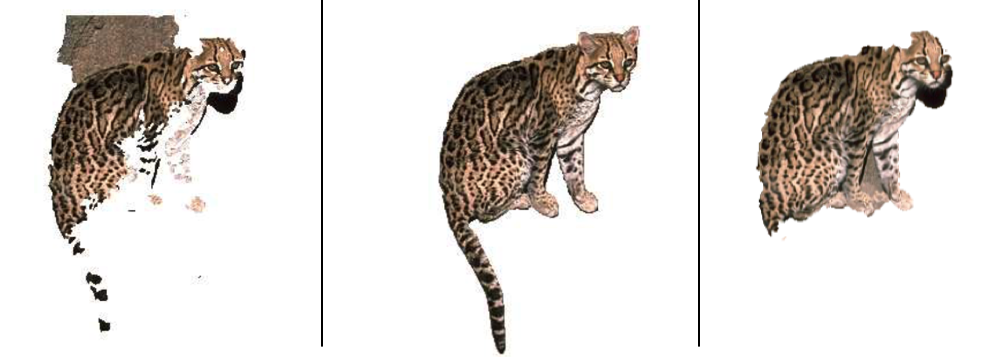
\includegraphics[width=\linewidth]{figures/grabCut/326038} \\
%     \vspace{1mm}
%     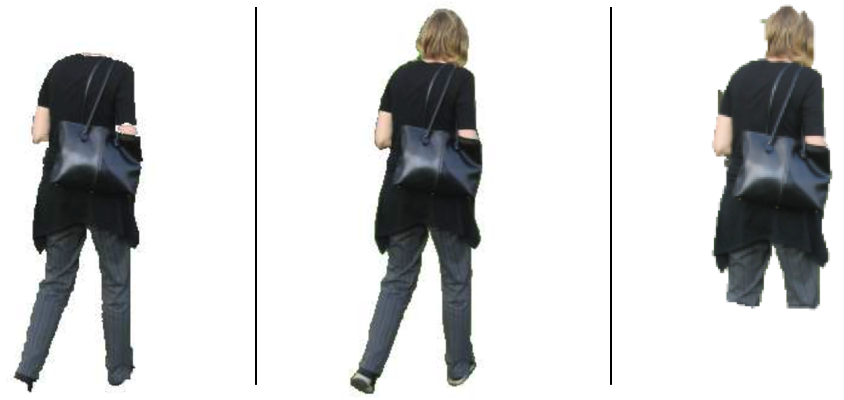
\includegraphics[width=\linewidth]{figures/grabCut/person5} \\
%     \vspace{1mm}
%     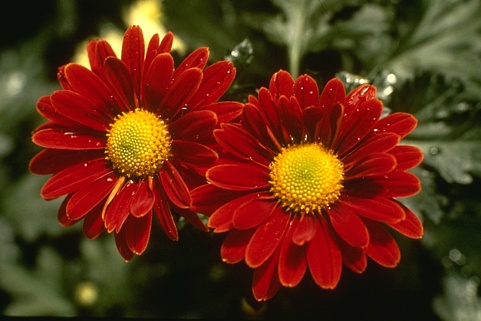
\includegraphics[width=\linewidth]{figures/grabCut/124080} \\
%     \vspace{1mm}
%     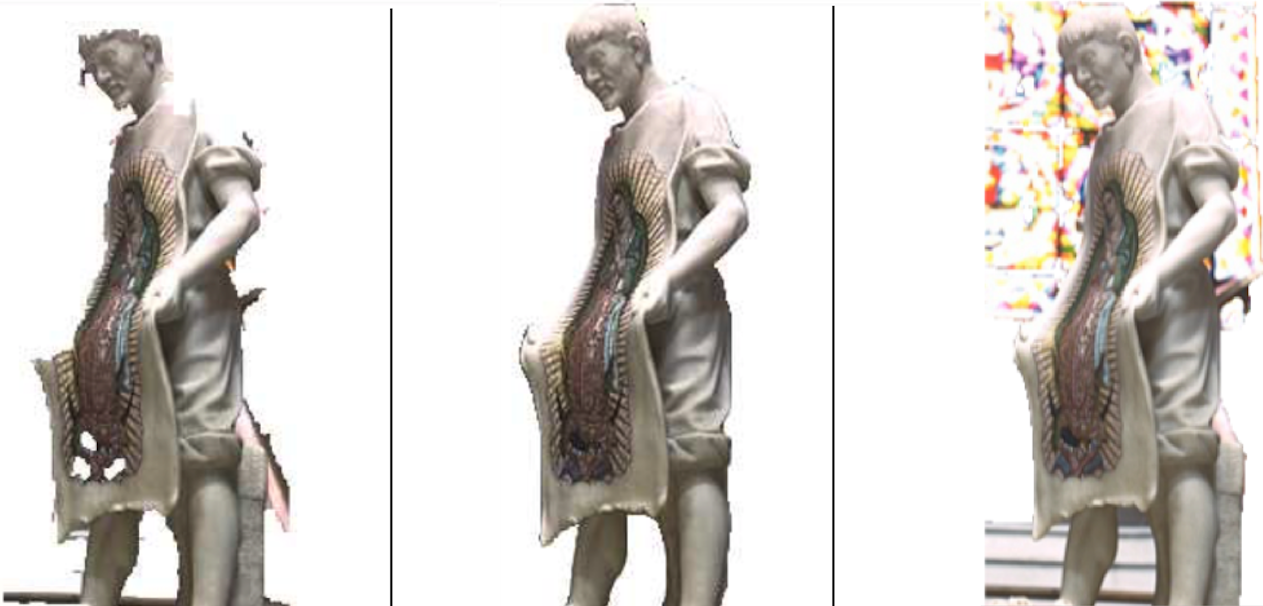
\includegraphics[width=\linewidth]{figures/grabCut/24077}
%       \begin{tabular}{c}
%         \begin{tabular}{p{0.24\linewidth}p{0.24\linewidth}p{0.24\linewidth}p{0.24\linewidth}}
%           {\small \hspace{5mm} (a)} & 
%           {\small \hspace{6.5mm} (b)} &
%           {\small \hspace{8mm} (c)} & 
%           {\small \hspace{9mm} (d)}
%         \end{tabular}
%     \end{tabular}
%     \caption{\label{fig:grabcut_results} Example results from our
%       GrabCut experiments. Shown are: (a) the image and bounding box,
%       (b) ground-truth segmentation, (c) baseline model output, and
%       (d) output from model with higher-order terms.}
%   \end{center}
% \
% end{figure}



\end{document}